\section{Algebraic Multigrid} \label{sec_amg}
\subsection{Introduction}
As mentioned earlier, the most common way to solve a SPD system is to use
conjugate gradient preconditioned with SSOR (PCG-SSOR). In this research, we
will compare the calculation time using PCG-SSOR with the time needed by CG 
preconditioned with an algebraic multigrid method. In \cite{amg_pn}, the authors 
used an algebraic multigrid method to precondition the Krylov solver for the 
even-parity finite element-spherical harmonics (FE-$P_N$) method. The AMG 
preconditioner resulted in a 60\% reduction in the solution time compared to 
ILU(0) preconditioning and even more reducion compared to SSOR preconditioning. 
Rather than writing our own AMG code, we will be testing the ML package 
\cite{ml_guide} from the Trilinos library and the AGMG code \cite{agmg_guide}. 
ML is a multigrid preconditioning package that uses a smoothed aggregation 
algebraic multigrid to build a preconditioner for a Krylov method. AGMG is an 
aggregation-based algebraic multigrid code written in Fortran 90.

Before explaining the differences between ML and AGMG, we need to explain the
how algebraic multigrid methods work. The first multigrid methods
developed were geometric multigrid used as stand-alone solvers. In many 
applications, they achieve the so-called ``textbook multigrid
efficiency'', i.e. ``the solution to the governing system of equations [is
attained] in a computational work that is a small multiple of the operation
counts associated with discretizing the system'' \cite{textbook_eff}. However, 
in many other applications, multigrid methods, and particularly algebraic 
multigrid methods, cannot achieve such efficiency \cite{k_cycle}. In
such cases, they are often used as preconditioner for Krylov subspace methods. 

Before solving a system of equations with a general multigrid method, we
explain how to solve it using a two-grid method. We want to
solve the following system:
\begin{equation}
  \bs{A}_f u_f = b_f
\end{equation}
define on the grid $\Gamma_f$ and that $\Gamma_c \subset \Gamma_f$. The 
two-grid algorithm is given by :
\begin{enumerate}
  \item $\nu_1$ pre-smoothing iterations using a smoother (Jacobi,
    Gauss-Seidel or ILU) and an initial guess $u_0$: $u = S^{\nu_1}(u_0,b_f)$
  \item Compute the residual on the fine grid $\Gamma_c$ and restrict it to
    the coarse grid $\Gamma_f$: $r_c = \bs{R}(b_f-\bs{A}_f u)$
  \item Solve the system on the coarse grid: $v=\bs{A}_c^{-1} r_c$
  \item Interpolate the coarse grid correction to the fine grid and add the
    correction to $u$: $u=u+\bs{P}v$
  \item $\nu_2$ post-smoothing iterations: $u = S^{\nu_2}(u,b_f)$
\end{enumerate}
When using AMG, the matrix $A_c$ on the coarse grid is given by the Galerkin
approximation:
\begin{equation}
  \bs{A}_c = \bs{R}\bs{A}_f \bs{P}
\end{equation}
where $\bs{P}$ is a prolongation matrix and $\bs{R}$ is a restriction matrix.
Solving the system $\bs{A}_c v = r_c$ on the coarse grid is generally very
expansive, therefore this step is recursively replaced by $\gamma$ two-grid
methods until the system can be efficiently inverted with a direct solver.
This yields the multigrid method. When $\gamma = 1$, respectively $\gamma =
2$, the multigrid method is said to use a $V-$cycle, respectively a $W-$cycle:
\begin{figure}[H]
  \centering
  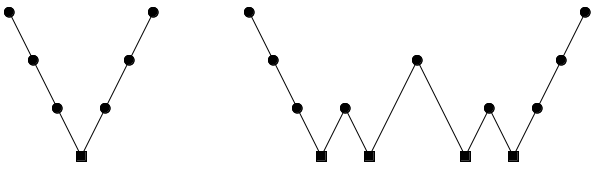
\includegraphics[width=0.5\textwidth]{./Dsa/v_w_cycles}
  \caption{$V-$ and $W-$ cycles.}
\end{figure}
A dot represents a smoothing operation. The grid transfer operators are 
symbolized by lines.

The main difference between geometric and algebraic multigrid is in the method
to coarsen the grid. Algebraic multigrid method only use the properties of the
matrix. Among the algebraic multigrid methods, there are three main different 
types: the classical Ruge-Stueben AMG, the plain aggregation AMG, and the
smoothed aggregation AMG. ML uses smoothed aggregation AMG and AGMG
uses plain aggregation AMG.  The coarsening step is the most important 
step because if the coarsening is too fast, the convergence rates will 
decrease. However, if the coarsening is too slow, a lot of memory may be 
required to solve the problem. 

\emph{Like geometric multigrid, AMG is based on smooth error. However, the
smoothness of the error cannot be determined geometrically anymore. Therefore,
the error is considered smooth when the smoother does not change the solution
significantly. Another very important concept for AMG is strongly dependence
of variable.
\definition{Given a threshold value of $0\leq \theta \leq 1$, the variable
$u_i$ strongly depends on the variable $u_j$ if:
\begin{equation}
  - a_{ij} \geq \theta \max_{k\neq i} \(-a_{ij}\) 
\end{equation}
}
Thus, $a_{ij}$ must be of the same order of magnitude than the largest
off-diagonal in equation $i$ or $j$ (we assume SPD or M matrix ?). 
\definition{If the variable $u_i$ strongly depends on the variable $u_j$,
then the variable $u_j$ strongly influences the variable $u_i$.}
The idea behind the strong dependence is that if the coefficient $a_{ij}$ is
large, then a small change in the $j^{th}$ variable will have a important
effect on the $i^{th}$ variable. Thus, it is probably a good idea to use the
$j^{th}$ variable to interpolate the $i^{th}$ variable or to couple these two
variables in an aggregate.}

\emph{The biggest difference between the interpolation and the aggregation
method is the coarsening step and the transfer operators. In interpolation
method, each variable of the coarse grid is also a variable in the fine grid.
At the opposite, the aggregation method aggregates the variables of the fine
grid in aggregates which are variables in the coarse grid. There is not simple
identification between the variables of the fine grid and the coarse grid.}

\subsection{Interpolation methods (Classical AMG)}

\red{With standard multigrid methods, smooth functions are geometrically or
  physically smooth, they have a low spatial frequency. With AMG because we do
  not have access to a physical grid, the sense of smoothness must be defined
  algebraically.\\
  The following bound must hold smooth error on average, that is, for most
  $i\in C$:
  \begin{equation}
    \sum_{j\neq i} \(\frac{|a_{ij}|}{a_{ii}}\) \(\frac{e_i-e_j}{e_i}\)^2 \ll 1
  \end{equation}
  The left side of the inequality is a sum of products of nonnegative terms.
  These products must be very small, which means that one or both of the
  factors in each product must be small. But if $e_i$ strongly depends on
  $e_j$, we know that $-a_{ij}$ could be comparable to $a_{ii}$. Therefore,
  for these strongly influencing $e_j$'s, it must be true that $e_i-e_j$ is
  small; that is $e_j\approx e_i$. We describe this by saying that smooth
  error varies slowly in the direction of strong connection. Thus, we have a
  justification for the idea that the fine-grid quantity $u_i$ can be
  interpolated from the coarse-grid quantity $u_j$ if strongly depends on $j$.
}

\red{Along with their corresponding norms $\|u\|_{\mc{H}^i} =
  \sqrt{u,u}_{\mc{H}^i}, i \in \{0,1,2\}$, the scalar products:
  \begin{align}
    & (u,v)_{\mc{H}^0} = (D u,v)_2\\
    & (u,v)_{\mc{H}^1} = (\bs{A} u,v)_2\\
    & (u,v)_{\mc{H}^2} = (D^{-1} \bs{A} u, \bs{A} v)_2
  \end{align}
  are needed. $D=diag(\bs{A})$ denotes the diagonal of $\bs{A}$. In some
  sense, these are discrete counters part of the $H^k$-Sobolev (semi-)norms.
  In algebraic error, an error $e$ is called smooth if it is slow to converge
  with respect to a smoother $S$. For example:
  \begin{equation}
    \|Se \|_{\mc{H}^1} \approx \|e\|_{\mc{H}^1}
  \end{equation}
  Depending on $\bs{A}$ an algebraically smooth error may well be highly
  oscillation geometrically. For typical relaxation schemes like Gauss-Seidel,
  the inequality:
  \begin{equation}
    \|S e\|_{\mc{H}^1}^2 \leq \|e \|_{\mc{H}^1}^2 \leq \|e \|_{\mc{H}^1}^2 -
    \alpha \|e\|_{\mc{H}^2}^2
  \end{equation}
  holds with $\alpha > 0$ (e.g. $\alpha = 1/4$). Therefore, a smooth error has
  to satisfy $\|e\|_{\mc{H}^2}\ll \|e\|_{\mc{H}^1}$. Applying the
  Cauchy-Schwartz inequality to $(\bs{A}e,e)_2 =
  \(D^{-1/2}\bs{A}e,D^{1/2}2\)_2$ shows:
  \begin{equation}
    \begin{split}
      \|e\|_{\mc{H}^1} &= \(D^{-1/2} \bs{A} e, D^{1/2} e\)_2\\
                       &= \|D^{-1/2} \bs{A} e \|_2 \|D^{1/2}\|_2 =
      \|e\|_{\mc{H}^2} \|e\|_{\mc{H}^0}
    \end{split}
  \end{equation}
  Therefore, $\|e\|_{\mc{H}^2} \ll \|e\|_{\mc{H}^1}$ implies $\|e\|_{\mc{H}^1}
  \ll \|e\|_{\mc{H}^0}$, or more explicitly: 
  \begin{equation}
    \begin{split}
      \(\bs{A}e,e\) &= \frac{1}{2} \sum_{i,j} -a_{ij}(e_i-e_j)^2 + \frac{1}{2}
      \sum_{i,j} a_{ij} e_i^2 + \frac{1}{2} a_{i,j} e_j^2\\
      &= \frac{1}{2} \sum_{i,j} -a_{ij}(e_i-e_j)^2 + \sum_i \(\sum_j
      a_{ij}\) e_i^2 \ll \sum_i a_{ii} e_i^2
    \end{split}
  \end{equation}
  For the important case $\sum_{i\neq j} |a_{i,j}| \approx a_{ii}$, this
  means that, on average for each $i$:
  \begin{align}
    &\frac{1}{2} \sum_{j\neq i} -a_{i,j}(e_i -e_j)^2 \ll a_{ii} e_i^2\\
    &\sum_{j\neq i} \frac{|a_{ij}|}{a_{ii}} \frac{(e_i-e_j)^2}{e_i^2} \ll 2
  \end{align}
  In other words, a smooth error generally varies slowly in the direction of
  strong connections, i.e. from $e_i$ to $e_j$ if $\frac{|a_{ij}|}{a_{ii}}$ is
  relatively large.
  \definition{$N_i^S$ denotes the set of all strongly connected neighbors of
    $v_i$:
    \begin{equation}
      N_i^S = \{v_j \in N+i | -a_{ij}\geq \theta \max_{m\neq i}(-a_{i,m}) \}
    \end{equation}
  }
  \definition{The interpolatory nodes $C_i$ are the strong $C-$node neighbors:
    \begin{equation}
      C_i = N_i^S \cap C
    \end{equation}
  }
  \definition{The noninterpolatory nodes $D_i$ are split into strong $D_i^S$
    and weak $D_i^W$ noninterpolatory nodes:
    \begin{align}
      &D_i = N_i\backslash C_i\\
      &D_i^S = D_i \cap N_i^S\\
      &D_i^W = D_i\backslash D_i^S
    \end{align}
  }
  Once again looking at :
  \begin{equation}
    a_{ii} e_i \approx -\sum_j a_{ij} e_j
  \end{equation}
  for a smooth vector $e$, we can expect that the interpolation of $e_j$,
  $v_j\in D_i$:
  \begin{equation}
    e_j = \frac{\sum_{v_k \in C_i} |a_{j,k}| e_k}{\sum_{v_m \in C_i} |A_{j,m}}
  \end{equation}
  is better for nodes $v_j$ which are strongly connected to the nodes in
  $C_i$. If we add nodes to $C_i$, very likely the quality of the
  interpolation increases. But on the other hand, the stencil sies of the
  prolongation and hence the stencil sizes of the coarse grid matrices and the
  numerical cost grows. Therefor, the following criteria are taken as
  guidelines in order to get good interpolations and a reasonable numerical
  complexity.
  \criterion{For each node $v_i\in F$, each node $v_j \in N_i^S$ should either
  be in $C$, or should be strongly connected to at least one node in
  $C_i$.\label{crit_1}}
  \criterion{$C$ should be a maximal subset of all nodes with the property
  that no two $C-$nodes are strongly connected to each other.\label{crit_2}}
  Criterion \ref{crit_1} shall ensure that the interpolation is good enough
  while criterion \ref{crit_2} enforces the coarsening algorithm to generate
  coarse grids with significantly less nodes than the fine grid. Since it is
  not always possible to satisfy strictly both criteria, criteria \ref{crit_2}
  is only taken as guideline while criterion \ref{crit_1} must be satisfied.\\
  The coarsening algorithm is divided into two steps. In the first step, a
  relatively quick $C-$node choice is performed. $C-$nodes are distributed
  uniformly over the grid attempting to enforce criterion \ref{crit_2}. In the
  second part the tentative $F-$nodes are tested to satisfy criterion
  \ref{crit_1} and the interpolation weights are computed. Tentative $F-$nodes
  not satisfying criterion \ref{crit_2} are labeled as $C-$nodes.}


\subsection{ML}
When using a smoothed aggregation scheme, the smoothed interpolation operators,
$\bs{P}_k$, are the transpose of the coarsening operators,
$\bs{R}_k=\bs{P}_k^T$. Therefore, when the $\bs{P}_k$ are built, the
coarsening is known. First, the graph of the matrix is constructed: if the element
$(i,j)$ or $(j,i)$ of the matrix is non-zero, an edge is built between the
vertex $i$ and the vertex $j$ \cite{ml_guide}. Second, the vertices are
aggregated. When using ML on a single processor, two aggregation schemes can
be used: the uncoupled scheme or the maximally independent sets (MIS) scheme. 
The uncoupled scheme tries to build aggregates of size $3^d$ where $d$ is the
dimension of the problem. The algorithm works as follows \cite{mis}:
\begin{description}
  \item[Step 1:] As long as there are points adjacent to an aggregate:
    \begin{enumerate}
      \item Choose a point which is not adjacent to an aggregate. This point
        is a new root point.
      \item Define a new aggregate as the root point and its neighbors 
    \end{enumerate}
  \item[Step 2:] Add all the points left to the existing aggregates or form a
    new aggregates with them
\end{description}
The MIS scheme used in ML applied the MIS algorithm \cite{graph_coloring} to
the graph produced by the square of the matrix $\bs{A}$. The goal is that all
the points belong to an aggregate without having to perform Step 2 of the
previous algorithm. These two coarsening schemes use a fixed ratio of 
coarsening between levels. Once the aggregation is done, a tentative
prolongator matrix, $\bs{\tilde{P}}_k$ is constructed \cite{mis}. A example of
$\bs{\tilde{P}}_k$ is given by:
\begin{equation}
  \bs{\tilde{P}}_k(i,j) = \left\{
  \begin{aligned}
    &1 &\textrm{if }i^{th}\textrm{ point is contained in }j^{th}\textrm{
    aggregate}\\
    & 0 &\textrm{otherwise}
  \end{aligned}
  \right.
\end{equation}
This tentative prolongator could be used as prolongator but smoothing it
allows to have a more robust scheme. Let $\bs{S}_k$ be a smoother, for example
damped Jacobi, the prolongator matrix is given by:
\begin{equation}
  \bs{P}_k = \bs{\tilde{S}}_k \bs{\tilde{P}}_k
\end{equation}

\red{The graph matrix can be altered by ignoring small values. In particular,
it is often preferential to ignore weak coupling during coarsening. The error
between weakly coupled points is generally hard to smooth and so it is best
not to coarsen in this direction. For example, when applying a Gauss-Seidel
smoother to a standard discretization of $u_{xx}+\epsilon u_{yy}=f$ with
$\epsilon \in [0,10^{6}]$, there is almost no coupling in the $y$ direction.
Consequently, simple smoothers like Gauss-Seidel do not effectively smooth the
error in this direction. If we apply a standard coarsening algorithm,
convergences rates suffer due to this lack of $y-$direction smoothing. There
are two principal ways to fix this: use a more sophisticated smoother or
coarsen the graph only in the $x$ direction. By ignoring the $y-$direction
coupling in the matrix graph, the aggregation phase effectively coarsens in
only the $x-$direction (the direction for which the errors are smooth)
yielding a significantly better multigrid convergence rates. In general, a
drop tolerance, $tol_d$, can be set such that an individual matrix entry,
$a_{ij}$ is dropped in the coarsening phase if: $|a_{ij}|\leq tol_d
\sqrt{|a_{ij}a_{jj}|}$. This dropped tolerance, whose default value is zero,
is set by ML\_AGGREGRATE\_SET\_THRESHOLD. When smoothing ML has a few ways to
determine the Jacobi damping parameter and each require some estimate of the
spectral radius of the discretization operator. The current default is to use
a few iterations of the power method (subspace size of two) to estimate this
value. However, if the matrix is SPD, CG should be used.}

\red{Pris de \cite{amg_unstruc}}\\
\red{We use the concept of strong connections to select our aggregates of
  nodes, which play a role similar to Ruge's coarse points. The theory for AMG
  was based on two-level estimates which do not give convergence bounds
  independent of the number of levels. The deterioration of convergence was
  indeed observed, and to defeat this, relatively many coarse point had to be
  selected, resulting in less attractive computational complexity. Our
  approach is based on the concept of smoothed aggregation. First, the set of
  nodes is decomposed into small mutually disjoint subsets. A tentative
  piecewise constant interpolation (in the discrete sense) is then defined
  using this decomposition. The final interpolation operator is obtained by
  smoothing the results of such piecewise constant interpolation. The coarse
  level operators are then defined variationally. The resulting method
  converges very fast for a wide range of problems including those with
  strongly anisotropic and discontinuous coefficients. In addition, the new
  method has remarkably low complexity since out typical coarsening ratio is
  about three in each dimension.}

\subsection{AGMG}
Unlike ML, in AGMG the prolongator is not smoothed which results in a
cheaper setup and a decrease of required memory \cite{agmg2}. However, as
explained previously, the scheme is less robust. To counteract this weakness, the
aggregation scheme is more complicated. Coarsening algorithms which control
the size of the aggregates tends to produce a few badly shaped aggregates.
Since the convergence of AMG is bounded by the worst aggregate, even a small 
number of badly shaped aggregates can have a huge impact on
the convergence. In AGMG, the aggregation algorithm has as input the upper
bound of the two-grid condition number. When the aggregates are constructed,
their quality is checked. Obviously, this increases the cost of the coarsening
and it is therefore important that the coarsening is fast enough. Since the 
algorithm does not control the size of the aggregates, it is difficult to 
control the speed of the coarsening. However, controlling the condition number
is much more interesting than controlling the coarsening speed. If the algorithm 
controls the condition number, it will not create bad aggregates but instead, it 
may create a few aggregates with a size below the target size. This obviously 
does not affect the efficiency of the method in an noticeable way \cite{agmg2}. 
In AGMG, the aggregation is done by a few passes of a pairwise aggregation 
algorithm. This allows the computation of the aggregate quality to remain very 
simple and to keep the cost per iteration low. The advantage of controlling the 
condition number becomes even more important when a $K-$cycle or Krylov-cycle is 
used instead of the more common $V-$ or $W-$cycles. The difference between the 
$K-$cycle and the $V-$ or $W-$cycle is that the $K-$cycle uses recursively a 
few iterations of a Krylov solver preconditioned by a coarser grid to solve 
the coarse grid problem in the two-grid algorithm \cite{k_cycle}. This scheme 
is nonlinear and requires, when the system is SPD, to use flexible CG 
\cite{fcg,fcg_2,fcg_3,fcg_4} as Krylov solver. The advantage of the $K-$cycle is 
an increased robustness compared to $V-$ and $W-$cycle. Even when the condition 
number of the two-grid method is large, the convergence properties of the 
$K-$cycle can be independent of the number of levels \cite{k_cycle}. The 
computational cost of $K-$cycle is about the same than the cost of the 
$W-$cycle. If the number of unknowns does not decrease sufficiently from one 
level to the next, the $K-$cycle at one level is replaced by a $V-$cycle at 
this same level.

\red{This motivates us to consider Krylov-basaed MG-cycles (or $K-$cycle, for
  short). With these cycles, the MG method is still based on the recursive use
  of a two-grid method, but the needed coarse-grid solve is defined by a few
  steps of a Krylov subspace iterative method with the already defined (by
  recursion) MG method on the previous (coarser) level as preconditioner. If
  $\mu$ inner iterations are performed at each level, we have more
  specifically a $K_{\mu}-$cycle preconditioner. Such an idea is not new; it
  has been used, also in a multilevel setting, for the so-called AMLI methods.
  The latter can be viewed as stabilized versions of the hierarchical basis
  methods. The stabilization comes from more than recursive calls of the
  preconditioner defined (by recursion) at a given level. Observe that the MG
  preconditioner defined in this way becomes a nonlinear operator and thus,
  the analysis of such techniques is not as straightforward.}

\red{Now, with the coarsening by aggregation, the prolongation is obtained
  from the agglomeration of the unknowns into $N-c$ nonempty disjoint sets
  $G_k$, $k=1,\hdots,n_c$ called aggregates. To each aggregate $G_k$ is
  associated one unknown at the next coarse level in the hierarchy. Besides,
  some unknowns can be also kept outside the coarsening process, and the
  corresponding (possibly empty) set is noted $G_0$; that is, $G_0$ gathers
  the unknowns that are not associated to any coarse unknown. As a result,
  $G_0$ together with $G_k$, $k=1,\hdots,n_c$ defines a partitioning of the
  index set $[1,n]$ which uniquely determines the prolongation $\bs{P}$: for
  $i=1,\hdots,n$ and $j=1,\hdots,n_c$:
  \begin{equation}
    \bs{P}_{ij} = \left\{
      \begin{aligned}
        1& \textrm{if }i\in G_j\\
        0& \textrm{otherwise}
      \end{aligned}
      \right.
  \end{equation}
  Hence a row of $\bs{P}$ is zero if and only if the corresponding unknown is
  in $G_0$, whereas the other rows have exactly one nonzero entry. Note that
  the entries in the coarse grid $\bs{A}_c = \bs{P}^T\bs{A} \bs{P}$ can be
  obtained from a simple summation process:
  \begin{equation}
    \bs{A}_{c,kl} = \sum_{i\in G_k} \sum_{j\in G_l} a_{ij}\ \ \
    k,l=1,\hdots,n_c
  \end{equation}
  It follows from this relation that if $\bs{A}$ is an $M-$matrix with
  nonnegative row sum, then $\bs{A}_c$ inherits from these properties. A naive
  approach when trying to build high quality aggregates of desired size would
  be to explore the matrix graph while testing all suitable aggregates. This
  is a costly strategy, because of the often important number of possibilities
  and the need to compute the quality estimate for each of them. An
  alternative would be to guess a few potentially interesting aggregates of
  targeted size or above and choose the most appropriate. Here, we follow this
  latter idea by considering an aggregation procedure based on a few passes of
  a pairwise algorithm, which attempts to group unknowns into pairs. When
  there are only two unknowns in $G$, the quality factor $\mu(G)$ reduces to
  an easy-to-compute function:
  \begin{equation}
    \mu(\{i,j\}) = \frac{-a_{ij}+\(\frac{1}{a_{ii}+s_i+2a_{ij}}+
    \frac{1}{a_{jj}+s_j+2a_{ij}}\)^{-1}}{-a_{ij}+\(\frac{1}{a_{ii}-s_i}
    +\frac{1}{a_{jj}-s_j}\)^{-1}}
  \end{equation}
  where $s_i = - \sum_{j\neq i} a_{ij}$ $\forall i \in U$. (Function involving
  only the off-diagonal entry connecting these two unknowns, their respective
  diagonal entries, and the sum of all off-diagonal elements in the
  corresponding rows). Whereas assessing $\mu(G)$ for large $|G|$ may become
  costly, it remains relatively cheap to check that $\mu(G)\leq
  \bar{\kappa}_{TG}$ for a given threshold. Indeed, this condition holds if
  and only if (to check):
  \begin{equation}
    \bar{\kappa}_{TG} \bs{A}_G - \bs{M}_G\(\bs{I}-\bs{1}_G \(\bs{1}_G^T
    \bs{M}_G\bs{1}_G\)^{-1}\bs{1}_G^T\bs{M}_G\)
  \end{equation}
  is nonnegative definite, which is true if and only if the Cholesky
  factorization if this matrix exists (i.e., no pivot is negative). Hence, the
  requirement (ii) if theorem 2.1 can be checked in only $\mc{O}(|G|^3)$
  operations. This is taken into account in the aggregation procedure, which
  allows to ensure that all aggregates satisfy the needed quality requirement,
  while avoiding an explicit computation of $\mu(G)$ for any subset $G$ with
  more than two unknowns. One first forms the set $G_0$ of unknowns that can
  be kept outside the aggregation. Next, one picks up an unknown at a time and
  searches, among its still unassigned neighbors, the one yielding the pair
  with the best quality. Then, it is checked whether or not this quality
  satisfies the acceptance criterion; if not, the unknown initially picked up
  remains unassociated in the coarse grid. To obtain large aggregates, we
  compute the auxiliary coarse grid matrix $\bs{\tilde{A}}$ corresponding to
  this initial pairwise aggregation. Then, we apply essentially the same
  algorithm to this matrix to form pairs of pairs; or, in subsequent applications,
  pairs of aggregates from the previous pass. The set $G_0$ has to remain the
  one initially defined during the first pass. Furthermore, the estimate
  $\tilde{\mu}(\{i,j\})$ used to assess the quality of the pair $\{i,j\}$ has
  to be adapted so as to correctly reflect the quality of the corresponding
  aggregate $\mu(G_i\cup G_j)$ in the original matrix. This is obtained by
  using the same formula but changing slightly the definition of
  $\tilde{s}_j$:
  \begin{equation}
    \tilde{s}_i = -\sum_{k\in G_i} \sum_{j\in G_i} a_{kj} \forall i \in U
  \end{equation}
  This change is needed to ensure that if $\tilde{\mu}(\{i,j\})$ is a lower
  bound on $\mu\(G_i \cup G_j\)$. It means that if $\tilde{\mu}(\{i,j\})$ is
  above the threshold, the pair should anyway be rejected because $\mu(G_i\cup
  G_j)$ cannot be smaller than $\bar{\kappa}_{TG}$. It also means that
  $\tilde{\mu}(\{i,j\})\leq \bar{\kappa}_{TG}$; however, as indicated above,
  this can be done by factorizing a $|G_i \cup G_j| \times |G_i \cup G_j|$
  matrix. An uncommon feature is that one can perform an arbitrary number of
  passes of pairwise aggregation without degrading the upper bound on the
  condition number. In practice, the process is stopped either if the
  specified maximal number of passes has been reached or once the coarsening
  factor is above a given target. So far, we did not discuss how to select the
  unknown in $U$ of the pairwise aggregation algorithms. For a given unknown
  $i$, there may be also several neighbors $j$ for which $\mu(\{i,j\})$ or
  $\tilde{\mu}\(\{i,j\}\)$ is minimal. If no priority rules are specified, the
  resulting aggregation will be sensitive to the ordering of the unknowns
  and/or the way off-diagonal entries are stored. Now, note that whereas the
  regularity of the aggregation is not an objective in itself, in practice it
  favors the coarsening speed at the subsequent coarse levels. Hence, after
  having tested several priority rules inspired, we found that the best
  results were obtained with a simple rule which primarily aims at producing
  regular aggregation patterns on regular grids. Somewhat surprisingly, good
  performance carries over problems on unstructured grids: results obtained
  with the rule given below are in such cases too at least as good as those
  obtained wit more sophisticated choices based on the dynamic update of
  unknowns' degree. The rule is as follows for the initial pairwise
  aggregation of the top level (fine grid) matrix. We first compute a
  Cuthill-McKee permutation \cite{cmk}; that is, we assign the number 1 to a
  node with minimal degree, and assign the next numbers to its neighbors
  ordered again by increasing degree; then, we number the unnumbered neighbors
  of the node that has just been given the number 2, still by increasing
  degree; we next proceed with the neighbors of node 3, and so on untill all
  nodes are numbered.} 
